\section{Domain Informed Oracle} 
\subsection{Architecture}
In this section, we lay the foundations of the architecture that combines the Domain Informed Oracle with 
reinforcement learning. Note that in our proposed architecture, we suppose Q-learning, a specific method to compute the policy in RL. 
It does not mean that our solution is specific to
Q-learning.\giselle{Last meeting you told me you are no longer using
Q-learning. Does this need to change?} 

\medskip 

\begin{figure}[H]
  \centering
  \begin{minipage}{.5\textwidth}
    \centering
    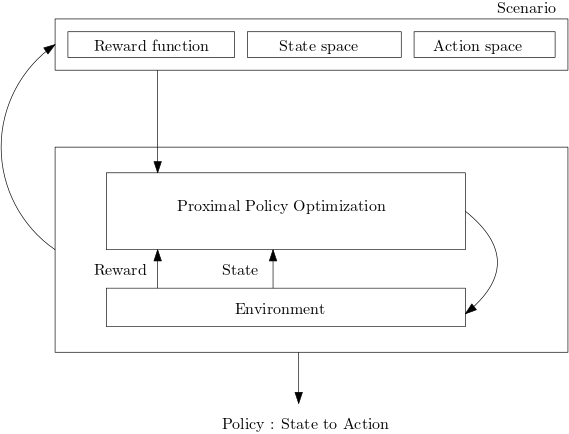
\includegraphics[width=1\linewidth]{figures/basicrl.png}
    \captionof{figure}{Reinforcement learning architecture}
    \label{fig:basicrl}
  \end{minipage}%
  \begin{minipage}{.45\textwidth}
    \centering
    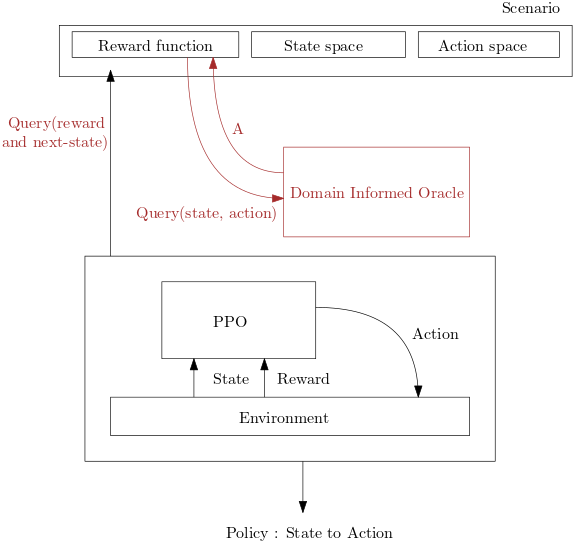
\includegraphics[width=1\linewidth]{figures/dio.png}
    \captionof{figure}{Dio+RL architectureg}
    \label{fig:diorl}
  \end{minipage}
\end{figure}


The diagram in Figure \ref{fig:basicrl}\giselle{This figure should
probably match Figure~\ref{fig:rl}. Note to self: discuss the diagram
on my whiteboard.} describes the basic routine of RL in more details. The environment defined by the scenario sends the current state 
to the Q-Learning algorithm. The agent chooses an action from the action space and sends it to the environment. This action affects the environment stepping it to some next state. 
The resulting state along its associated reward is computed from the reward function and step function formalized in the scenario. Thus, in the next iteration, the 
agent receives the reward from its previous action which it uses to improve its policy and continues with its training starting from the computed next state.  

\medskip 

The architecture in Figure \ref{fig:diorl}\giselle{Note to self:
discuss this figure} introduces DIO in the feedback loop. It is kept independent of the RL module. Precisely, when the scenario is query-ed for the reward and 
the resulting next state of a (state, action) pair, rather than computing the reward using the reward function, the latter is able to query DIO. The result of this query is $A$ which we keep 
obscure. The fundamental idea is that $A$ is used to inform the reward function when it is tasked with computing the reward. 

\subsection{Specifications} \label{scspecs}
DIO is a logic programming based module that takes the query from the reward function and returns $A$, a judgment that the scenario awaits to update its reward function. The judgment is obscured as it is a choice of the scenario, 
independent of the DIO implementation. In the following, we will define $A$ by its behavior, rather than its type. To do so, we will walk through the routine in the diagram of Figure \ref{fig:diospecs}.


\begin{figure}[H]
  \centering
  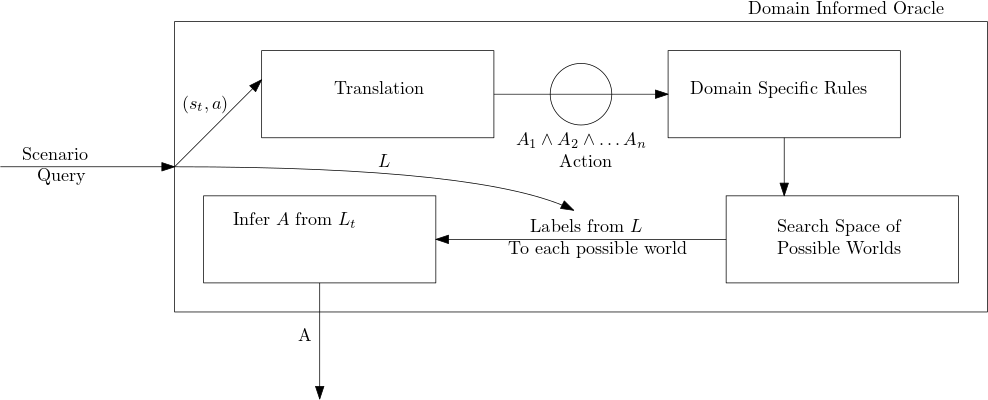
\includegraphics[scale=0.46]{figures/diospecs.png}
  \caption{Domain Informed Oracle routine}
  \label{fig:diospecs}
\end{figure}
\giselle{Perhaps this figure corresponds too much to what is
implemented, and makes the general idea more complicated than it
should be.}

\begin{enumerate}
  \item The scenario queries DIO. It sends $(s_t, a)$, the state at time $t$ and the action. It also sends $L : s \rightarrow t$ where $t$ is a sum of types: 
        $t \equiv t_1 + t_2 .. + t_n$. For instance, consider our previous example of the chess game and let the scenario define good openings as "desirable" and random openings as 
        "undesirable". Thus $t \equiv d + ud$ where $d$ is equivalent to desirable and $ud$ to undesirable. 
  \item The first step of DIO is a translation $T : \mathbb{R}^n
  \rightarrow t_1 \times t_2 \times ... t_n$\giselle{You use the same
  $t_i$ as in the previous item, but I suspect these are different.
  Propositions usually have type $\omicron$.} that takes in the state
  vector $s_t$ and returns a conjunction of propositions $P = A_1 \wedge
  A_2 \wedge ... \wedge A_n$. This is our set of ground facts.
  \item P is passed alongside the action to the domain specific rules defined in DIO. 
  \item Using step semantics, DIO generates possible worlds up to a given time $t'$. Note that given the stochasticity of the environment, there is no certainty on
        whether the worlds expected by DIO will necessarily happen. Consider Figure \ref{fig:diosim}.
  \item Those possible worlds, equivalent to states, can be
  transformed using $L$ to $t$.\giselle{Is this implemented in python
  or problog?}
  \item At the last step, DIO ends up with a set $S$ of $t$ that defines the labels of all the possible worlds.
  \item The last step is left as an inference depending on how the the judgment for deciding a final $A$ from $S$ 
        is formulated. For instance, we can consider a rule where if most of the possible worlds are undesirable, then let $A$ be undesirable.
  \item Finally, $A$ is passed to the scenario. Note then that $A : t$. 
\end{enumerate}

\begin{figure}
  \centering
  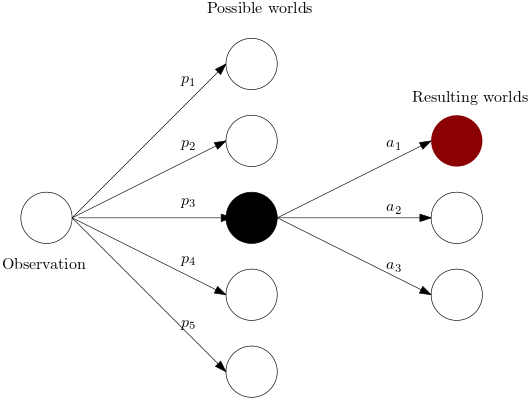
\includegraphics[scale=0.55]{figures/scworlds.png}
  \caption{Game Tree Simulation by DIO}
  \label{fig:diosim}
\end{figure}

Observe how this does not guarantee that the reward function will be informed in a meaningful way.
To that end, we need to consider (1) what are the specifications of a 'good' reward function, (2) what conditions should be set 
on the domain specific rules and $L$ provided by the scenario, (3) how to define a systematic way for the scenario to use 
this information. Those considerations are left for future
investigations.\giselle{You have good results. How are you using the
information to compute the reward? Unrelated: you should be careful
here not to give the impression that you are just adding one layer to
the problem of reward shaping (the problem before is how to write a
reward function given a state vector, the problem now is how to write
a reward function given $A$).} 
 

\subsection{Modules Interactions}
\label{sec:modules}
In practice, we consider the following modules and their interactions as shown in \ref{fig:mods}.

\begin{enumerate}
  \item \textbf{World Rules} defining the rules governing the world. This is domain-dependent and implemented 
        in a logic programming file, i.e. we are able to define the next step via step semantics.
  \item \textbf{World Knowledge Base} defining the ground facts which describe the world at a given time step. This module is 
        continuously updated to account for the dynamics of the
        state.\giselle{Calling it ``World'' sounds static, this is
        actually the description of the state as propositional facts,
        correct?} 
  \item \textbf{Labels} i.e., textual ``norms'' corresponding to an
  iteration of the state. In practice, they are predicates, e.g. \textit{crash :- obs(X,Y), agent(X,Y)}. 
                    Those labels have probabilities associated with
                    them.\giselle{Do you mean \emph{crash} or all the
                    predicates in the rule? Is this a judgment on the
                    state?}
  \item \textbf{Translation Unit} defining the translation from state to ground facts and from labels to a numerical value, e.g. if the predicate crash is true with $P = 0.25$, then the reward shaped is $r + -0.25$. 
  \item \textbf{Reinforcement Learning} is our independent module that does not make assumption on the algorithm chosen for RL.
\end{enumerate}


\begin{figure}[H]
  \centering
  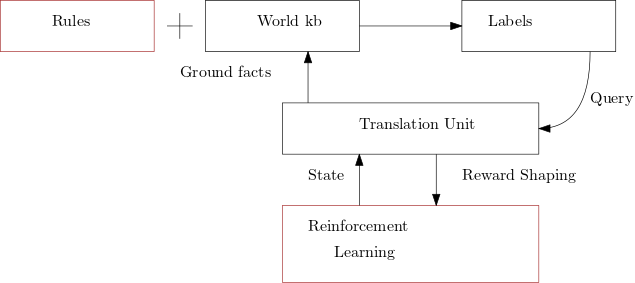
\includegraphics[scale=0.55]{figures/dynamics.png}
  \caption{Modules \& Interactions}
  \label{fig:mods}
\end{figure}
\giselle{I feel like this superseeds (and it is better than
Figure~\ref{fig:diospecs})}

Figure \ref{fig:mods} describes the interactions of the different modules. Precisely, 
given the rules and the world knowledge base at a given time $t$, we are able 
to produce the corresponding label, i.e. the query over a predicate. The predicate is fed 
into the Translation Unit (TU) that transforms the predicate to a numerical value that is given to the Reinforcement Learning 
as a reward shaping $r'$ added to the original reward given by the
environment.\giselle{Adding to the original reward... This might
explain the success of the experiments :)} As a result of the RL action, the next state is given 
to TU that translates it into Ground facts to update the world
knowledge, thus restarting the loop.
